%% img/SetsResolution.tex
%% Copyright 2019 Andrea Berlingieri
%
% This work may be distributed and/or modified under the
% conditions of the LaTeX Project Public License, either version 1.3
% of this license or (at your option) any later version.
% The latest version of this license is in
%   http://www.latex-project.org/lppl.txt
% and version 1.3 or later is part of all distributions of LaTeX
% version 2005/12/01 or later.
%
% This work has the LPPL maintenance status `maintained'.
%
% The Current Maintainer of this work is Andrea Berlingieri.
%
% This work consists of all files listed in manifest.txt
\documentclass{standalone}

\usepackage{TikzStyle}
\usepackage{mystyle}

\begin{document}
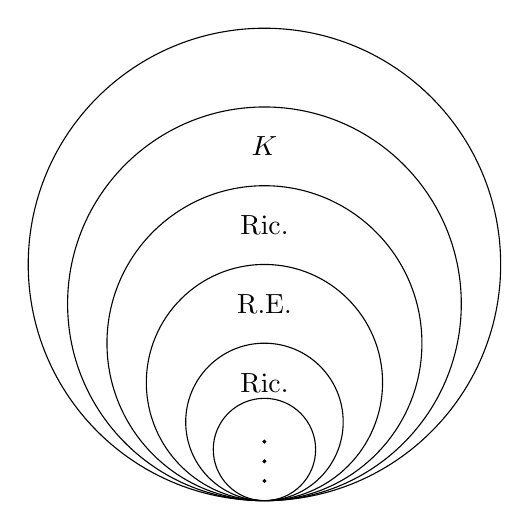
\begin{tikzpicture}[point/.style={draw,shape=circle,radius=1pt,inner sep=0pt,fill}]
    \draw (0,0) circle [radius=3cm];
    \draw (0,-0.5) circle [radius=2.5cm];
    \draw (0,-1) circle [radius=2cm];
    \draw (0,-1.5) circle [radius=1.5cm];
    \draw (0,-2) circle [radius=1cm];
    \draw (0,-2.35) circle [radius=0.65cm];
    \node at (0,2.5) {$\Nat$};
    \node at (0,1.5) {$K$};
    \node at (0,0.5) {Ric.};
    \node at (0,-0.5) {R.E.};
    \node at (0,-1.5) {Ric.};
    \foreach \y in {-2.25,-2.5,-2.75}
    {
        \node[point] () at (0,\y) {};
    }
\end{tikzpicture}
\end{document}
